\input preamble

\title{OCaml}
\subtitle{Знакомство}

\date{18 апреля 2020 г.}

\begin{document}

\begin{frame}
  \titlepage{}

  \begin{textblock*}{4cm} (13cm,5.1cm)
  
\includegraphics[height=3.5cm]{./images/ag.png}
  \end{textblock*}
\end{frame}

\begin{frame}
  \frametitle{\$ whois Pavel Argentov}
  \large
  \vspace{8mm}
  \begin{columns}
    \begin{column}{8cm}
      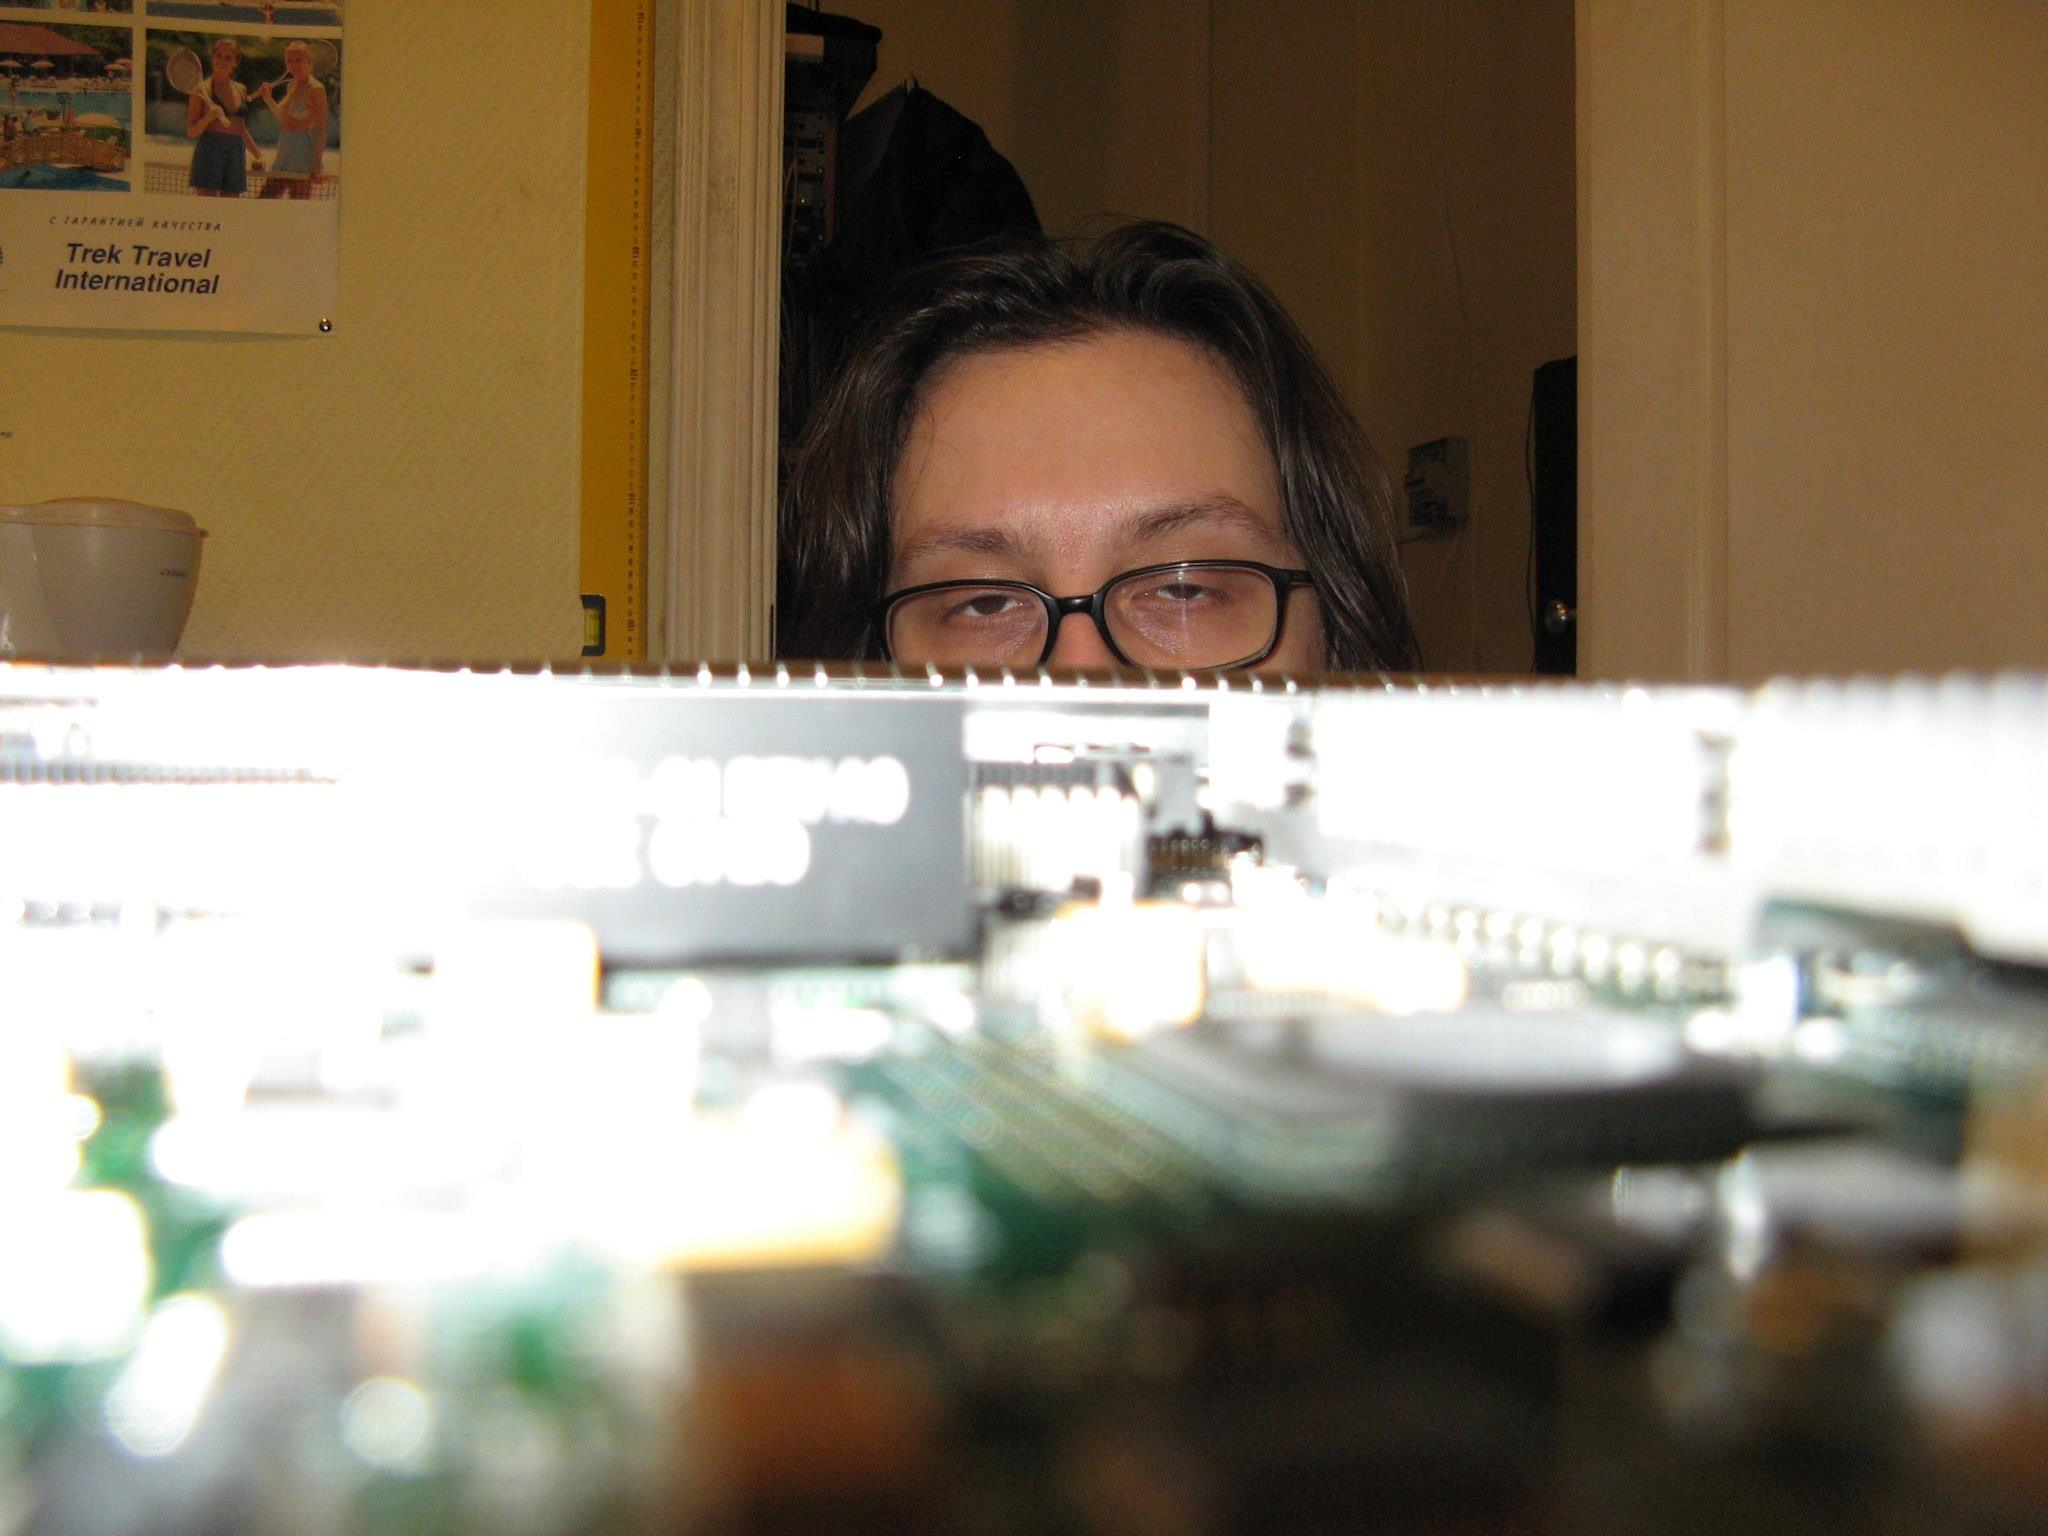
\includegraphics[width=8cm,keepaspectratio]{./images/ag_cisco.jpg}
    \end{column}

    \begin{column}{5cm}
      \begin{itemize}
        \item Hello, IT:\@ 3 г.
        \item Telecom, ISP:\@ 10 л.
        \item Webdev, backend 2012 --- \dots
      \end{itemize}
    \end{column}
  \end{columns}
\end{frame}

\begin{frame}
  \frametitle{\$ whois Pavel Argentov}
  \large
  \vspace{8mm}
  \begin{columns}
    \begin{column}{8cm}
      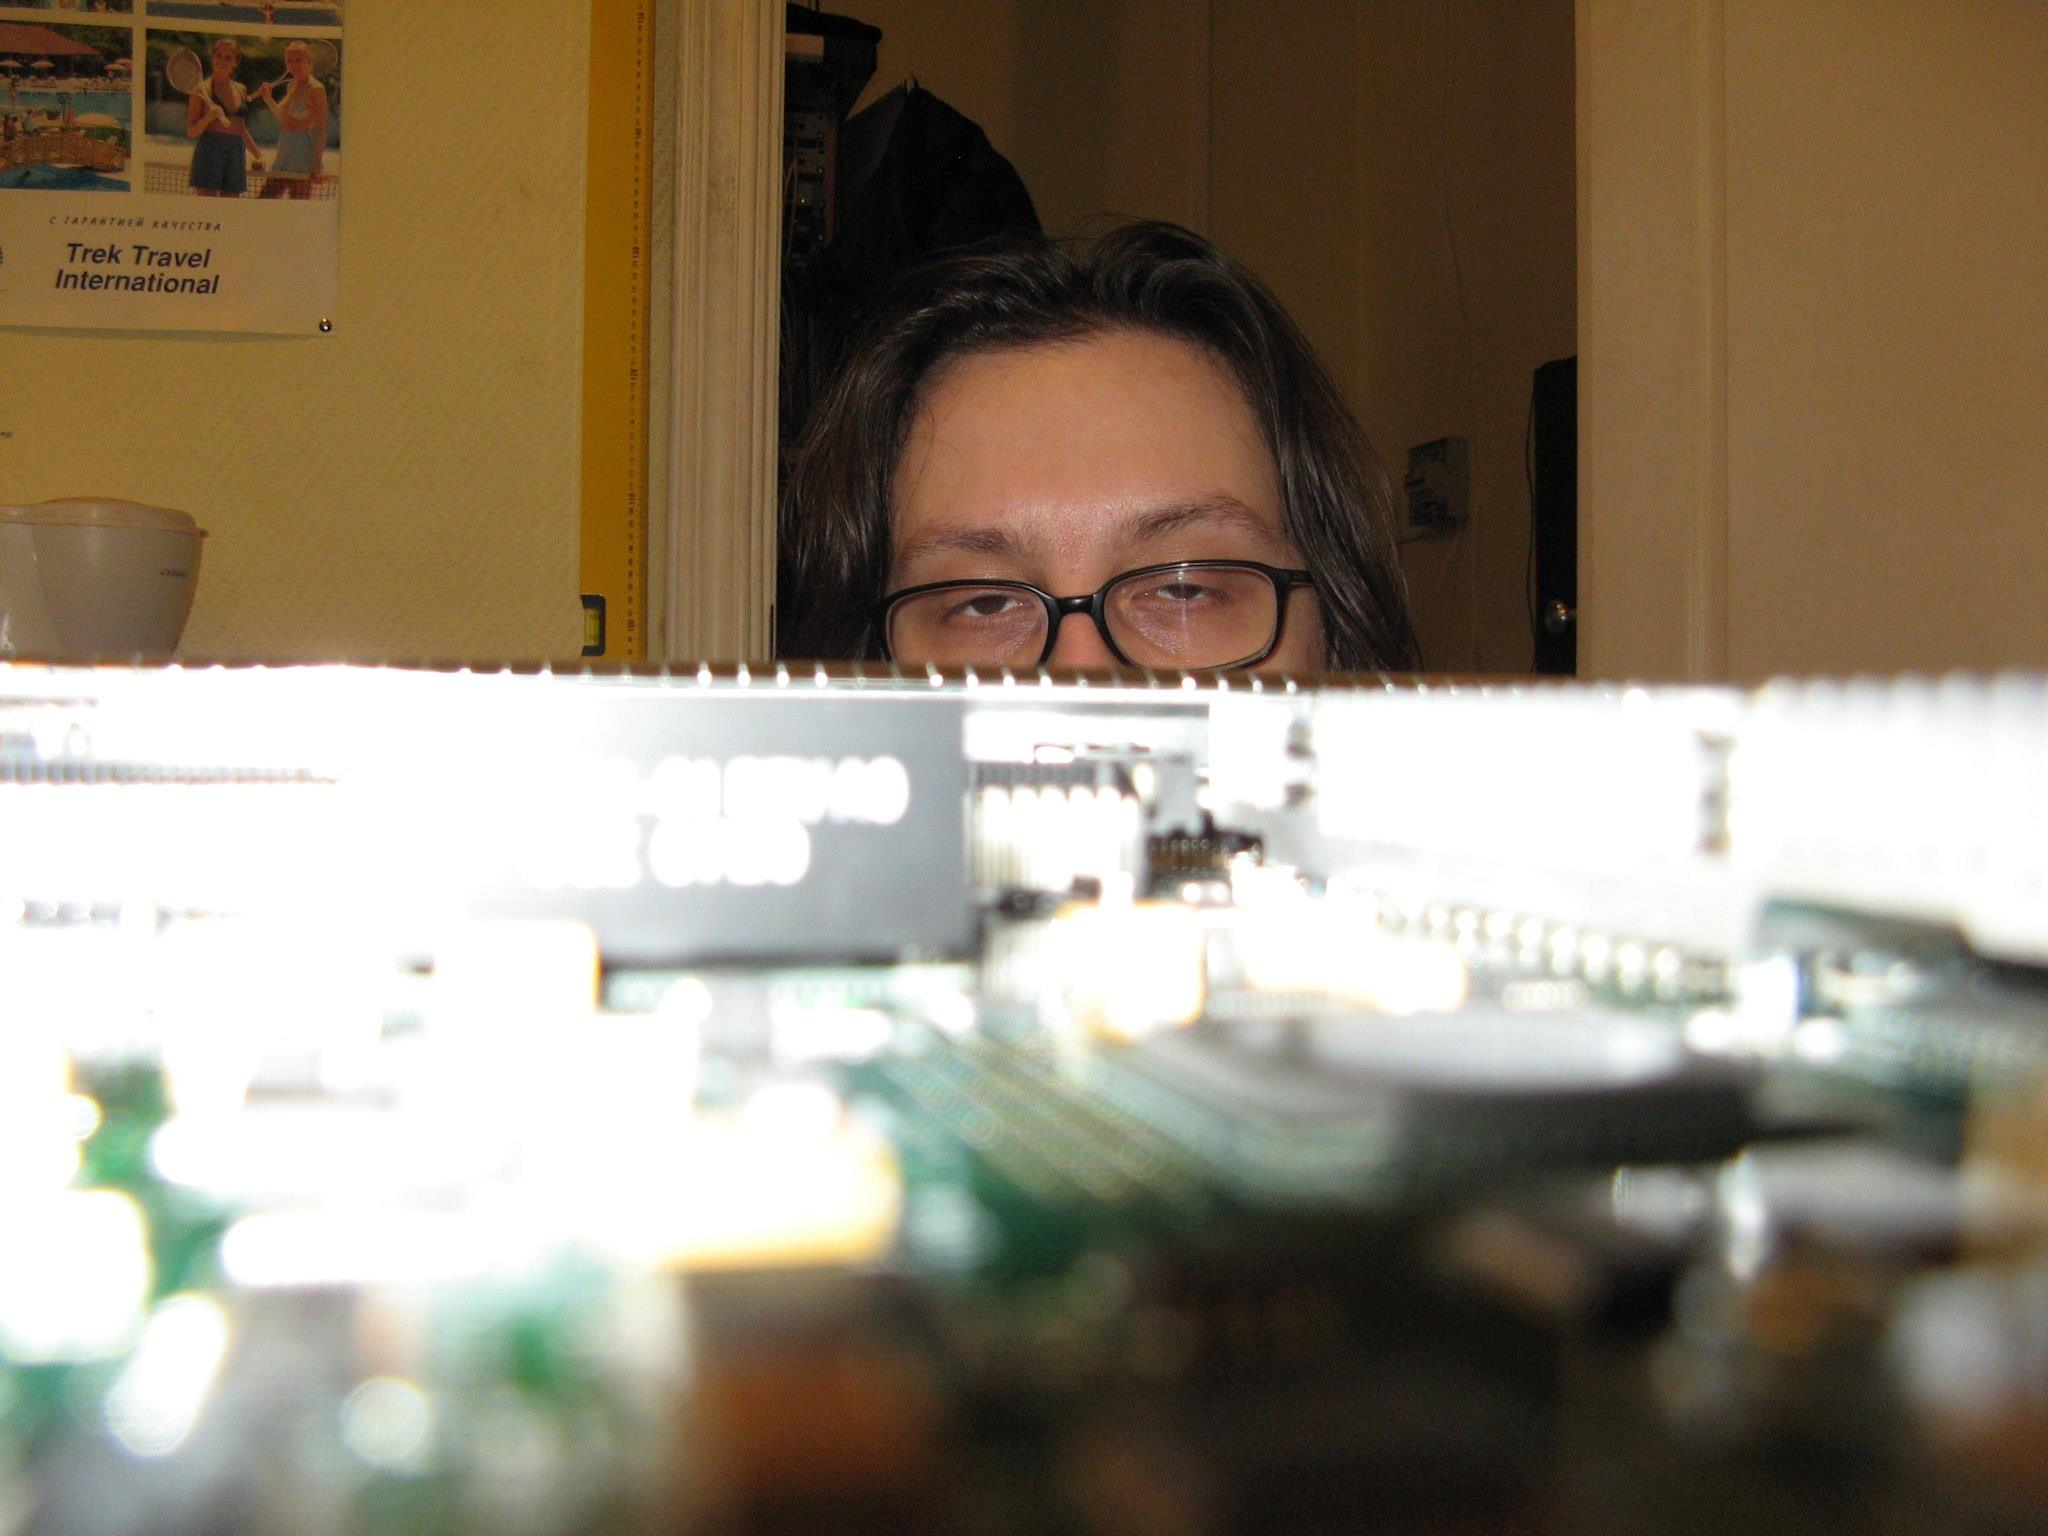
\includegraphics[width=8cm,keepaspectratio]{./images/ag_cisco.jpg}
    \end{column}

    \begin{column}{5cm}
      
\includegraphics[width=5cm,keepaspectratio]{./images/ocaml_logo.png}
      где-то в 2005
    \end{column}
  \end{columns}
\end{frame}

\begin{frame}
  \frametitle{\$ cat disclaimers}
  \begin{center}
    \LARGE
    \begin{itemize}
      \item Не буду защищать OCaml \pause
      \item Не буду сравнивать OCaml и Haskell \pause
      \item Не буду продавать ФП
    \end{itemize}
  \end{center}
\end{frame}

\begin{frame}
  \frametitle{\$ cat disclaimers}
  \begin{center}
    \Large <<Я каску на стройке нашёл>>\\
    \vspace{2mm}
    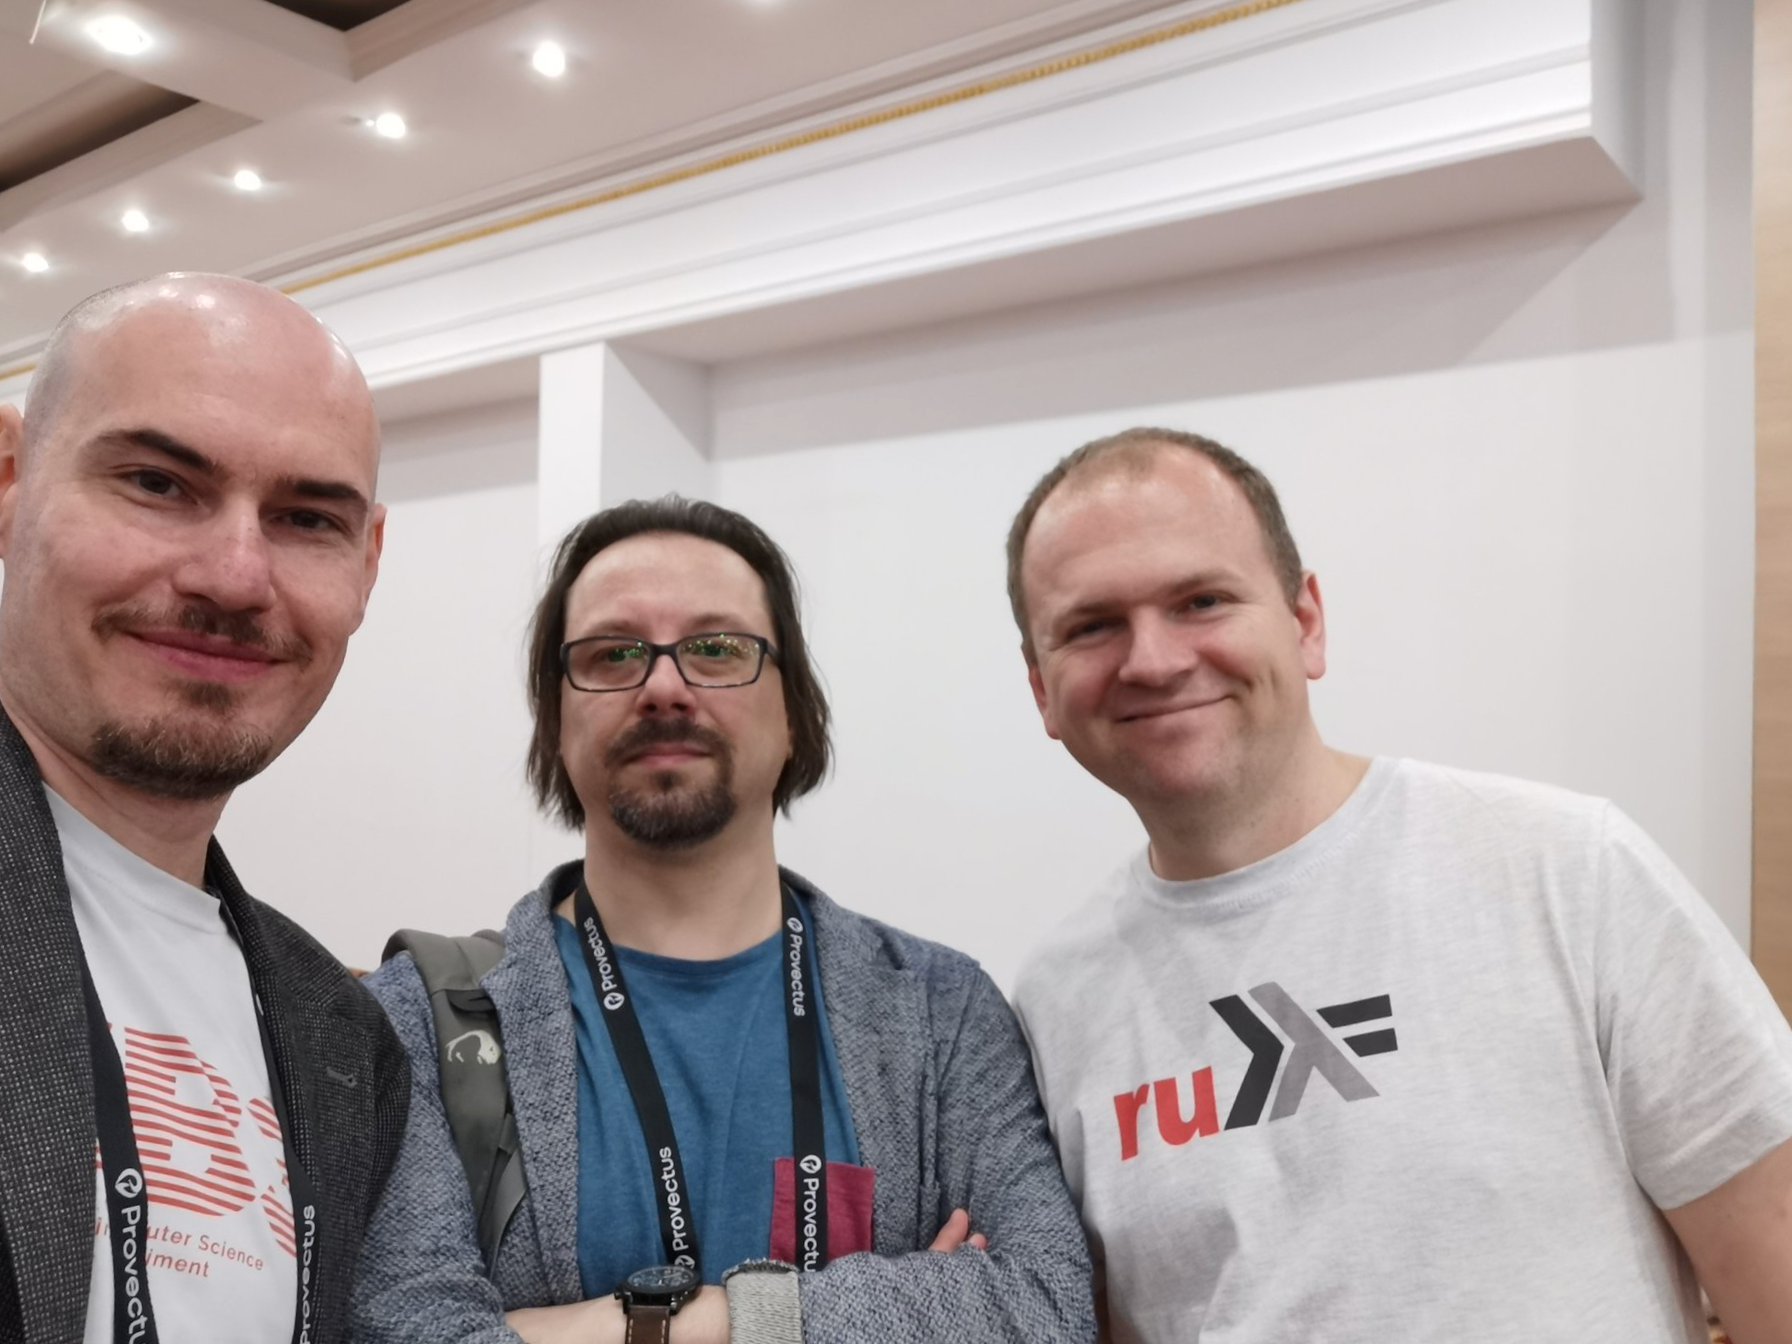
\includegraphics[width=8cm,keepaspectratio]{./images/arrested.png}
  \end{center}
\end{frame}

\begin{frame}
  \frametitle{OCaml: кому это выгодно?}
  \large
  \begin{columns}
    \begin{column}{6cm}
      \begin{enumerate}
        \item Утилиты
        \begin{itemize} \normalsize
          \item Unison
          \item Mldonkey
        \end{itemize}
        \pause

        \item Системный софт
        \begin{itemize} \normalsize
          \item Xen
          \item MirageOS
        \end{itemize}
        \pause

        \item Языки
        \begin{itemize} \normalsize
          \item Coq
          \item Flow
          \item ReasonML
          \item BuckleScript
          \item Hack
        \end{itemize}
      \end{enumerate}
    \end{column}
    \pause

    \begin{column}{6cm}
      \Large
      \begin{itemize}
        \item Bloomberg L.P.
        \item Jane Street Capital
        \item Citrix Systems
        \item Facebook
        \item Docker
      \end{itemize}
    \end{column}
  \end{columns}
\end{frame}

\begin{frame}
  \frametitle{OCaml: кто это сделал?}

  \begin{itemize}
    \Large
    \item 1980s, The Origin, ML\\
    \normalsize
    Robin Milner (LCF, ML), G\'{e}rard Huet (Lisps),\\
    Guy Cousineau (ADT, PM, CAM + ML = Caml) \pause
    \Large
    \item 1987--1992, The First Implementation\\
    \normalsize
    Ascander Suarez, Pierre Weis, Michel Mauny, LLM3 (Le\_Lisp) \pause
    \Large
    \item 1990s, Caml Light\\
    \normalsize
    Xavier Leroy (BC impl'n), Damien Doligez (memory management)
  \end{itemize}
\end{frame}

\begin{frame}
  \frametitle{OCaml: кто это сделал?}

  \begin{itemize}
    \Large
    \item 1996--2000, Objective Caml\\
    \normalsize
    Didier R\'{e}my,  J\'{e}r\^{o}me Vouillon (OO subsystem)\\
    Jacques Garrigue (polymorphic methods, labeled/optional arguments, polymorphic variants) \pause
    \Large
    \item 2000--\dots, OCaml\\
    \normalsize
    Xavier Leroy, BDFL
  \end{itemize}
\end{frame}

\begin{frame}
  \frametitle{OCaml: кто это сделал?}

  \vspace{5mm}
  \begin{center}
    
\includegraphics[width=5cm,keepaspectratio]{./images/qr-ocaml-history.png}
  \end{center}
\end{frame}

\begin{frame}[fragile]
  \frametitle{OCaml: экосистема}

  \Large Компилятор(-ы): версионирование
  \normalsize
  \begin{textcode}
  $ opam switch list-available
  # Listing available compilers from repositories:
  # Name              # Version
  ocaml-base-compiler 3.07
  <...>
  ocaml-variants      4.11.0+trunk
  ocaml-variants      4.11.0+trunk+afl
  ocaml-variants      4.11.0+trunk+flambda
  \end{textcode}
\end{frame}

\begin{frame}
  \frametitle{OCaml: экосистема}

  \Large Компилятор(-ы): бэкенды
  \large
  \begin{itemize}
    \item Bytecode
    \item Native\\
      \normalsize IA-32, X86-64 (AMD64), Power, SPARC, ARM, ARM64
    \item JS\\
      ocsigen/js-of-ocaml
  \end{itemize}
\end{frame}

\begin{frame}[fragile]
  \frametitle{OCaml: экосистема}

  \Large Build systems: Dune
  \scriptsize
  \begin{schemecode}
  (executable
   (name rpiterm)
   (public_name rpiterm)
   (preprocess (pps lwt_ppx))
   (libraries cmdliner
              rpiterm_lib
              prometheus-app.unix)
   (flags (-safe-string))
   (ocamlopt_flags (:standard (:include ocamlopt_flags.sexp))))

  (rule
   (targets ocamlopt_flags.sexp)
   (deps (:discover config/discover.exe))
   (action (run %{discover})))
  \end{schemecode}
\end{frame}

\begin{frame}
  \frametitle{OCaml: экосистема}

  \Large Менеджеры пакетов
  \begin{itemize}
    \large
    \item OPAM
      \normalsize
      \begin{itemize}
        \item global \& local compiler switching
        \item dependencies isolation in local switch
        \item env sandboxing
      \end{itemize}
      \pause
    \large
    \item Esy
      \normalsize
      \begin{itemize}
        \item package.js driven (npm style)
        \item uses OPAM
        \item env sandboxing
        \item artifacts caching
        \item Nix style
      \end{itemize}
  \end{itemize}
\end{frame}

\begin{frame}
  \frametitle{OCaml: экосистема}

  \Large Editors integration: Merlin
  \begin{center}
    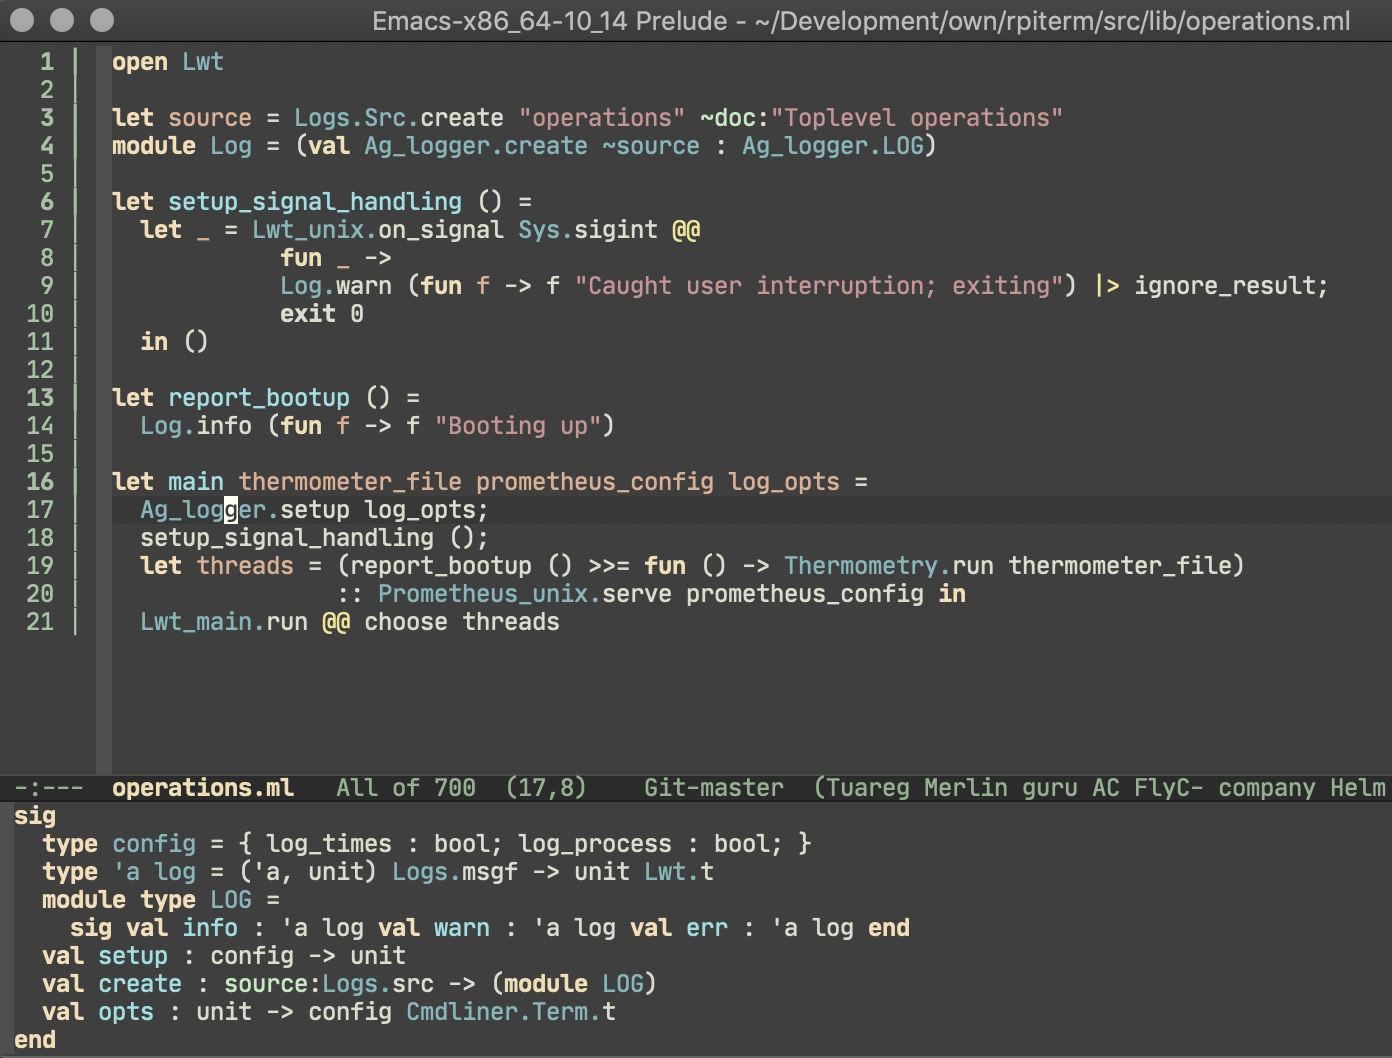
\includegraphics[height=6cm,keepaspectratio]{./images/merlin-shot-emacs.png}
  \end{center}
\end{frame}

\begin{frame}
  \frametitle{OCaml: экосистема}

  \Large REPL: Utop
  \begin{center}
    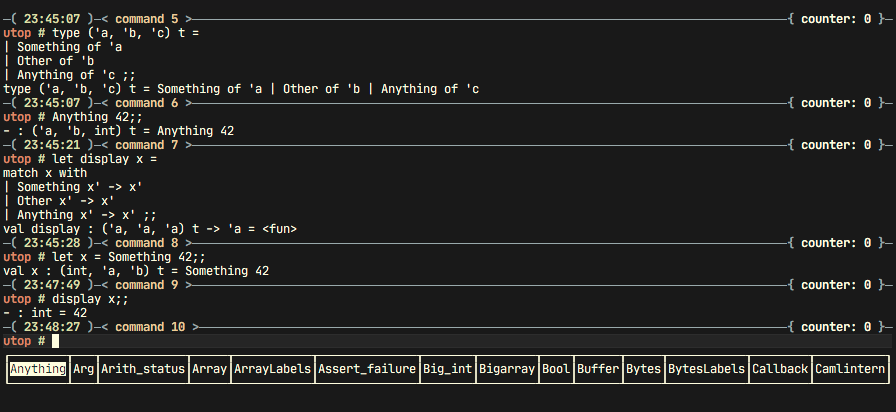
\includegraphics[height=55mm,keepaspectratio]{./images/utop-shot.png}
  \end{center}
\end{frame}

\begin{frame}
  \frametitle{OCaml: экосистема}

  \begin{center}
    \LARGE Awesome OCAML\\
    \vspace{3mm}
    
\includegraphics[width=5cm,keepaspectratio]{./images/qr-awesome-ocaml.png}
  \end{center}
\end{frame}

\begin{frame}
  \frametitle{OCaml: напишем маленькую программку\dots}

  \begin{center}
    \Large argent-smith/rpiterm\\
    \vspace{3mm}
    
\includegraphics[width=5cm,keepaspectratio]{./images/qr-rpiterm.png}
  \end{center}
\end{frame}

\begin{frame}[fragile]
  \frametitle{OCaml: напишем маленькую программку\dots}

  \Large <<Термометр>> для Raspberry Pi (ARM64)
  \normalsize
  \begin{textcode}
  [INF] operations: Booting up
  [INF] thermometry: Got thermometer value as 68.218
  [INF] thermometry: Got thermometer value as 67.680
  [INF] thermometry: Got thermometer value as 68.756
  [INF] thermometry: Got thermometer value as 67.680
  \end{textcode}
\end{frame}

\begin{frame}
  \frametitle{OCaml: напишем маленькую программку\dots}

  \Large <<Термометр>> для Raspberry Pi (ARM64)
  \normalsize
  \begin{itemize}
    \item \large Поток 1
    \begin{enumerate}
      \item Прочитать float из файла с температурой
      \item Отдать его в Prometheus-exporter
      \item Поспать 5 секунд
      \item Повторить
    \end{enumerate}

    \item \large Поток 2 (Prometheus exp.)
    \begin{enumerate}
      \item Ждать http-запрос
      \item Отдать ответ
      \item Повторить
    \end{enumerate}
  \end{itemize}
\end{frame}

\begin{frame}
  \frametitle{OCaml: языки}

  \LARGE
  \begin{enumerate}
    \item Язык типов \pause
    \item Язык модулей \pause
    \item Язык ФП \pause
    \item Язык ИП \pause
    \item Язык ООП
  \end{enumerate}
\end{frame}

\begin{frame}[fragile]
  \frametitle{OCaml: язык типов}

  \small
  \begin{ocamlcode}
type nonrec 'a ref = 'a ref = { mutable contents : 'a; }
type nonrec 'a option = None | Some of 'a
type nonrec int
type wtf = Well 'a | Nope
type metric_type =
  Counter | Gauge | Summary | Histogram
type sample = {
  ext    : string;
  value  : float;
  bucket : (LabelName.t * float) option;
}
type ft = string option -> int -> int option
  \end{ocamlcode}
\end{frame}

\begin{frame}[fragile]
  \frametitle{OCaml: язык модулей}

  \small
  \begin{ocamlcode}
module type THERMOMETER = sig
  val read_temperature :
    ?t_file : string option -> unit -> float result Lwt.t
end
module Mockup : THERMOMETER = struct
  let read_temperature ?(t_file = None) () =
    return @@ Ok (36600.0 /. 1000.0)
end
let get_thermometer_value _file =
  let module T = Thermometer.Linux in
  let%lwt thermometer_value = T.read_temperature () in
  ...
  \end{ocamlcode}
\end{frame}

\begin{frame}[fragile]
  \frametitle{OCaml: язык модулей}

  \small
  \begin{ocamlcode}
module type X_int = sig val x : int end

module Increment (M : X_int) : X_int = struct
  let x = M.x + 1
end

module Three = struct let x = 3 end

module Four = Increment(Three)

Four.x - Three.x  (* - : int = 1 *)
  \end{ocamlcode}
\end{frame}

\begin{frame}[fragile]
  \frametitle{OCaml: язык модулей}
  \footnotesize
  \begin{ocamlcode}
module type LOG = sig
  val info : 'a log
  val warn : 'a log
  val err : 'a log
end
let create ~source =
  let module Src_log = (val Logs.src_log source : Logs.LOG) in
  let module Log = struct
      let info msgf = Src_log.info msgf |> return
      and warn msgf = Src_log.warn msgf |> return
      and err msgf = Src_log.err msgf |> return
    end
  in
  (module Log : LOG)
  \end{ocamlcode}
\end{frame}

\begin{frame}[fragile]
  \frametitle{OCaml: язык ФП}

  \large
  Иммутабельность, first-class функции, карринг

  \footnotesize
  \begin{ocamlcode}
open Prometheus

let namespace = "node"
and subsystem = "hwmon"

let chip_temperature =
  let help = "Hardware monitor for temperature (input)"
  and label_name = "sensor" in
  Gauge.v_label ~help ~label_name ~namespace ~subsystem "temp_celsius"
  \end{ocamlcode}
\end{frame}

\begin{frame}[fragile]
  \frametitle{OCaml: язык ФП}

  \large LET <<на выброс>> и точка входа
  \footnotesize
  \begin{ocamlcode}
let () =
  match Term.eval (operation, info) with
  | `Error _ -> exit 1
  | _ -> exit 0

let setup_signal_handling () =
  let _ = Lwt_unix.on_signal Sys.sigint @@
    fun _ ->
      Log.warn (fun f -> f "Caught user interruption; exiting")
      |> ignore_result;
      exit 0
  in ()
  \end{ocamlcode}
\end{frame}

\begin{frame}[fragile]
  \frametitle{OCaml: язык ФП}

  \large Паттерны (и ppx)
  \footnotesize
  \begin{ocamlcode}
let read_temperature ?(thermometer_file = None) () =
  match thermometer_file with
  | None -> return @@ Error No_thermometer_file
  | Some filename ->
     let open Lwt_io in
     let read_float channel =
       let%lwt str = read_line channel in
       return @@ Ok ((float_of_string str) /. 1000.0)
     in
     try%lwt
           with_file ~mode:input filename read_float
     with
     | exn -> return @@ Error exn
  \end{ocamlcode}
\end{frame}

\begin{frame}[fragile]
  \frametitle{OCaml: язык ФП}

  \large Рекурсия (и монада)
  \footnotesize
  \begin{ocamlcode}
let rec run thermometer_file =
  Lwt_unix.sleep 5.0
  >>= (fun () -> get_thermometer_value @@ Some thermometer_file)
  >|= Prometheus.Gauge.set @@ Metrics.chip_temperature "soc_chip_temp"
  >>= fun () -> run thermometer_file
  \end{ocamlcode}
  \vfill
\end{frame}

\begin{frame}[fragile]
  \frametitle{OCaml: язык ИП}

  \large Мутабельность: ссылки
  \footnotesize
  \begin{ocamlcode}
type 'a ref = { mutable contents : 'a }

let ref x = { contents = x }
let x = ref 1

let (:=) r x = r.contents <- x
let (!) r = r.contents
x := !x + 1

!x (* - : int = 2 *)
  \end{ocamlcode}
  \vfill
\end{frame}

\begin{frame}[fragile]
  \frametitle{OCaml: язык ИП}

  \large Мутабельность: структуры (note the ``;'')
  \footnotesize
  \begin{ocamlcode}
type client_info =
 { addr: Unix.Inet_addr.t;
   port: int;
   user: string;
   credentials: string;
   mutable last_heartbeat_time: Time_ns.t;
   mutable last_heartbeat_status: string;
 }

let register_heartbeat t hb =
  t.last_heartbeat_time   <- hb.Heartbeat.time;
  t.last_heartbeat_status <- hb.Heartbeat.status_message
  \end{ocamlcode}
  \vfill
\end{frame}

\begin{frame}[fragile]
  \frametitle{OCaml: язык ИП}

  \large Циклы
  \footnotesize
  \begin{ocamlcode}
let quit_loop = ref false in
while not !quit_loop do
  print_string "Have you had enough yet? (y/n) ";
  let str = read_line () in
  if str.[0] = 'y' then
    quit_loop := true
done

for j = 0 to last_col do
  m3i.(j) <- inner_loop last_row 0 m1i m2 j
done
  \end{ocamlcode}
  \vfill
\end{frame}

\begin{frame}[fragile]
  \frametitle{OCaml: язык ООП}

  \footnotesize
  \begin{ocamlcode}
class ['a] stack =
  object (self)
    val mutable list = ( [] : 'a list )  (* instance variable *)
    method push x =                      (* push method *)
      list <- x :: list
    method pop =                         (* pop method *)
      let result = List.hd list in
      list <- List.tl list;
      result
    method peek =                        (* peek method *)
      List.hd list
    method size =                        (* size method *)
      List.length list
  end
  \end{ocamlcode}
  \vfill
\end{frame}

\begin{frame}[fragile]
  \frametitle{OCaml: язык ООП}

  \begin{ocamlcode}
let s = new stack

s#push 3.0
s#pop         (* - : float = 3. *)
  \end{ocamlcode}
  \vfill
\end{frame}

\begin{frame}[fragile]
  \frametitle{OCaml: язык ООП}

  \large Immediate objects
  \small
  \begin{ocamlcode}
let o =
  object
    val mutable n = 0
    method incr = n <- n + 1
    method get = n
  end

val o : < get : int; incr : unit > = <obj>
  \end{ocamlcode}
  \vfill
\end{frame}

\begin{frame}
  \frametitle{Thnx}

  \begin{center}
    \LARGE @argent\_smith\\
    \vspace{3mm}
    
\includegraphics[width=5cm,keepaspectratio]{./images/qr-lecture.png}\\
  \end{center}
\end{frame}

\end{document}
